%%%%%%%%%%%%%%%%%%%%%%%%%%%%%%%%%%%%%%%%%
% Beamer Presentation
% LaTeX Template
% Version 1.0 (10/11/12)
%
% This template has been downloaded from:
% http://www.LaTeXTemplates.com
%
% License:
% CC BY-NC-SA 3.0 (http://creativecommons.org/licenses/by-nc-sa/3.0/)
%
%%%%%%%%%%%%%%%%%%%%%%%%%%%%%%%%%%%%%%%%%

%----------------------------------------------------------------------------------------
%   PACKAGES AND THEMES
%----------------------------------------------------------------------------------------

\documentclass{beamer}

\mode<presentation> {}

% The Beamer class comes with a number of default slide themes
% which change the colors and layouts of slides. Below this is a list
% of all the themes, uncomment each in turn to see what they look like.

%\usetheme{default}
%\usetheme{AnnArbor}
%\usetheme{Antibes}
%\usetheme{Bergen}
%\usetheme{Berkeley}
\usetheme{Berlin}
%\usetheme{Boadilla}
%\usetheme{CambridgeUS}
%\usetheme{Copenhagen}
%\usetheme{Darmstadt}
%\usetheme{Dresden}
%\usetheme{Frankfurt}
%\usetheme{Goettingen}
%\usetheme{Hannover}
%\usetheme{Ilmenau}
%\usetheme{JuanLesPins}
%\usetheme{Luebeck}
%\usetheme{Madrid}
%\usetheme{Malmoe}
%\usetheme{Marburg}
%\usetheme{Montpellier}
%\usetheme{PaloAlto}
%\usetheme{Pittsburgh}
%\usetheme{Rochester}
%\usetheme{Singapore}
%\usetheme{Szeged}
%\usetheme{Warsaw}

% As well as themes, the Beamer class has a number of color themes
% for any slide theme. Uncomment each of these in turn to see how it
% changes the colors of your current slide theme.

%\usecolortheme{albatross}
%\usecolortheme{beaver}
%\usecolortheme{beetle}
%\usecolortheme{crane}
%\usecolortheme{dolphin}
%\usecolortheme{dove}
%\usecolortheme{fly}
%\usecolortheme{lily}
%\usecolortheme{orchid}
%\usecolortheme{rose}
%\usecolortheme{seagull}
%\usecolortheme{seahorse}
%\usecolortheme{whale}
%\usecolortheme{wolverine}

%\setbeamertemplate{footline} % To remove the footer line in all slides uncomment this line
%\setbeamertemplate{footline}[page number] % To replace the footer line in all slides with a simple slide count uncomment this line

%\setbeamertemplate{navigation symbols}{} % To remove the navigation symbols from the bottom of all slides uncomment this line


\usepackage{graphicx} % Allows including images
\usepackage{booktabs} % Allows the use of \toprule, \midrule and \bottomrule in tables
\usepackage{xcolor}   % Allows for change of font color
\usepackage{algorithm}
\usepackage{mathtools}
\usepackage{algpseudocode}
\usepackage{bm}
\usepackage{calc}
\usepackage{etoolbox}
\usepackage{array}
\usepackage{amssymb}% http://ctan.org/pkg/amssymb
\usepackage{pifont}% http://ctan.org/pkg/pifont
\setbeamertemplate{mini frames}{}
\usepackage{scrextend}
\usepackage{animate}
\changefontsizes{10pt}
%----------------------------------------------------------------------------------------
%   TITLE PAGE
%---------------------------------------------------------------------------------------

\title[NYC-Taxi]{STA 208 Project Report - NYC Taxi Data Pickup Prediction} % The
% short title appears at the bottom of every slide, the full title is only on the title page

\author{Xingtai Li, Guicheng Wu, Wenhao Wu} % Your name
\institute[UC Davis]{ % Your institution as it will appear on the bottom of every slide, may be shorthand to save space
  University of California, Davis \\ % Your institution for the title page
  \medskip
  \textit{gchwu, xtali, wnhwu@ucdavis.edu} % Your
  % email address
}
\date{\today} % Date, can be changed to a custom date

%\AtBeginSection[]
%{
%  \begin{frame}<beamer>
%    \frametitle{Outline for Section \thesection}
%    \tableofcontents[currentsection]
%  \end{frame}
%}

\setbeamertemplate{theorems}[numbered]
\pretocmd{\part}{\setcounter{theorem}{0}}{}{}
\newtheorem{proposition}[theorem]{Proposition}

\newcommand{\cmark}{\ding{51}}%
\newcommand{\xmark}{\ding{55}}%

\begin{document}
\begin{frame}
  \titlepage % Print the title page as the first slide
\end{frame}

\begin{frame}
  \frametitle{Content} % Table of contents slide, comment this block out to remove it
  \tableofcontents % Throughout your presentation, if you choose to use \section{} and \subsection{} commands, these will automatically be printed on this slide as an overview of your presentation
\end{frame}

\section[Introduction]{Introduction}
\begin{frame}
  \frametitle{Background}
  \begin{itemize}
    \item Objective: predicting the number of taxi pickups within a certain period of time
    and a neighborhood in New York City.
    \item Potential Applications: more efficient cab dispatch, trip planning,
    traffic monitoring, etc.
    \item Related projects:
    \begin{enumerate}
      \item MIT Big Data Challenge, 2013.
      \item Todd W. Schneider, ``Analyzing 1.1 Billion NYC Taxi and Uber
      Trips, with a Vengeance,'' 2015.
      \item Di-Tech Challenge, 2016.
    \end{enumerate}
  \end{itemize}
\end{frame}

\section[Methodology]{Methodology}
\begin{frame}
  \frametitle{Data Sets Processing Techniques}
  \begin{block}{Data Sets}
    \begin{itemize}
      \item NYC TLC Taxi Data Year 2014 (25GB), 177312293 complete records.
      \item NOAA daily average temperature and precipitation measured by New
      York Central Park Belvedere Tower observing station.
    \end{itemize}
  \end{block}
 \begin{block}{Processing Techniques}
    \begin{itemize}
      \item Data import: PostgreSQL+PostGIS via SQLAlchemy+GeoAlchemy.
      \item Machine learning: scikit-learn.
      \item Visualization: Matplotlib+Basemap.
    \end{itemize}
  \end{block}
\end{frame}

\begin{frame}
  \frametitle{Demo: NYC TLC Taxi Data}
  Pickups/hr/mi$^2$ in 24 hours (averaged over 365 days)
  \begin{columns}[c]
    \column{.5\textwidth}
    \animategraphics[loop,controls,width=\linewidth]{3}{./figs/density_by_ct_yellow/density_movie_yellow-}{0}{23}

    \column{.5\textwidth}
    \animategraphics[loop,controls,width=\linewidth]{3}{./figs/density_by_ct_green/density_movie_green-}{0}{23}
  \end{columns}
\end{frame}

\begin{frame}
  \frametitle{Demo: NYC TLC Taxi Data}
  Time series analysis: hourly number of pickups ($365\times 24$)
  \begin{figure}
    \centering
    \begin{minipage}[b]{1.0\columnwidth}
      \centering
      \centerline{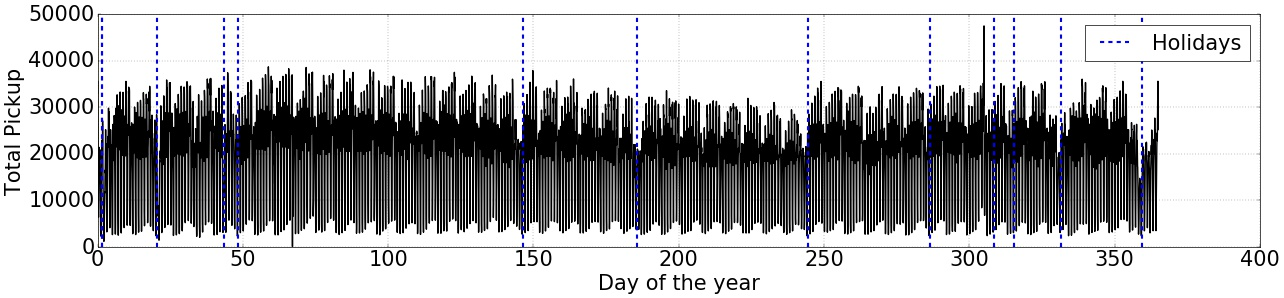
\includegraphics[width=\linewidth]{./figs/total_pickup_time.jpg}}
    \end{minipage}
    \hfill
    \begin{minipage}[b]{1.0\columnwidth}
      \centering
      \centerline{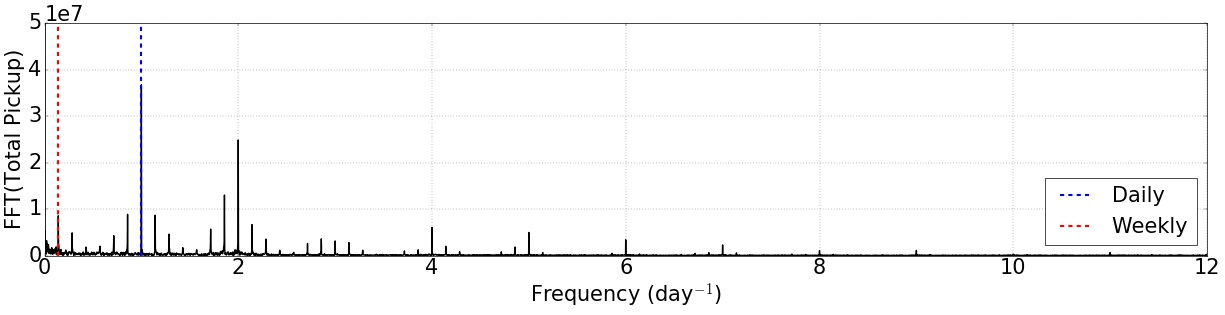
\includegraphics[width=\linewidth]{./figs/total_pickup_freq.jpg}}
    \end{minipage}
    \caption{Temporal and frequency pattern of the total pickup count.}
    \label{fig:temporal_freq}
  \end{figure}
\end{frame}

\begin{frame}
  \frametitle{Feature Selection}
  \begin{table}[H]
    \renewcommand{\arraystretch}{1.3}
    \caption{Feature selection.}
    \label{table:feature}
    \centering
    \begin{tabular}{ | c | c | c |}
      \hline      
      Feature name & Data Type & Meaning \\
      \hline
      pickup gid & categorical & The id of pickup neighborhood. \\
      \hline
      pickup dow & categorical & Day of week (0..6) \\
      \hline  
      pickup hour & categorical & Hour of pickup (0..23)\\
      \hline
      temperature & numerical & Daily Temperature\\
      \hline
      precipitation & numerical & Daily Precipitation\\
      \hline
      holiday & categorical & True/False\\
      \hline 
      count\_1 & numerical & pickups at previous hour\\
      \hline
    \end{tabular}
  \end{table}
  Categorical features are encoded $\longrightarrow$ a total of 35 features
  
  (7 (DOW)+24 (hr)+temperature+precipitation+holiday+count\_1).
\end{frame}

\begin{frame}
  \frametitle{Machine Learning Models}
  \begin{enumerate}
    \item Linear regression.
    \item Lasso.
    \item Support ridge regression.
    \item Bayesian linear regression.
    \item Decision tree.
  \end{enumerate}
\end{frame}

\begin{frame}
  \frametitle{Performance Metrics}
  \begin{itemize}
    \item For each neighborhood (NTA) a regression model is trained independent
    of other NTAs.
    \item Performance metric: $R^2$ coefficient of determination
    \begin{align}
      R^2(y, \hat{y}) = 1 - \frac{\sum_{i=0}^{n} (y_i - \hat{y_i})}{\sum_{i =
      0}^{n} (y_i - \overline{y})},\,\overline{y} = \frac{1}{n}\sum_{i=0}^{n}y_i
    \end{align}
    as well as mean squared error (MSE)
  \end{itemize}
\end{frame}

\section[Results]{Results}

\subsection[Model Selection]{Model Selection}
\begin{frame}
  \frametitle{Model Comparison (1/3)}
  \begin{itemize}
    \item Training/testing set split: 80\% vs 20\%.
    \item Only the 26 NTAs with the average number of pickups per hour per
    square mile greater than 100 are studied.
  \end{itemize}
  \begin{table}[H]
    \renewcommand{\arraystretch}{1.3}
    \caption{Training and testing results of the 5 regression models for Upper
    East Side-Carnegie Hill}
    \label{table:feature}
    \centering
    \begin{tabular}{ | c | c | c | c |}
      \hline      
      Regressor & Parameter & $R^2$ & RMSE \\
      \hline
      Linear  & - &  0.8987 & 128.5 \\
      \hline
      Lasso & $\alpha = 0.01$ & 0.9005 & 130.51 \\
      \hline  
      SVR & rbf kernel, $C=10^5$ & 0.6710 & 241.61\\
      \hline
      Bayesian Ridge & $\alpha=10^{-5}$,$\lambda=10^{-6}$ &0.9009 & 131.06\\
      \hline
      Decision Tree & max length =100,min leaf = 10 & 0.9241 & 104.8\\
      \hline
    \end{tabular}
  \end{table}
\end{frame}

\begin{frame}
  \frametitle{Model Comparison (2/3)}
  \begin{figure}[!t] 
    \centering
    \includegraphics[width=0.7\columnwidth]{./figs/r_2.png}
    \caption{Comparison of the regressors in $R^2$ scores for all 26
    selected NTAs.
    }
    \label{fig:comparison_r2}
  \end{figure}
\end{frame}

\begin{frame}
  \frametitle{Model Comparison (3/3)}
  \begin{figure}[!t] 
    \center
    \includegraphics[width=0.7\columnwidth]{./figs/mse.png}
    \caption{Comparison of the regressors in MSE for all 26
    selected NTAs.}
    \label{fig:comparison_mse}
  \end{figure}
\end{frame}

\subsection[Decision Tree]{Examination on The Decision Tree Model}

\begin{frame}
  \frametitle{Training Curve}
  Focusing on the decision tree for Upper East Side-Carnegie Hill (gid=27).
  \begin{figure}[H] 
    \center
    \includegraphics[width=0.9\columnwidth]{./figs/learning_curve.png}
    \caption{Learning curve for the decision tree.}
    \label{fig:learning_curve}
  \end{figure}
\end{frame}

\begin{frame}
  \frametitle{Weights of Features}
  \begin{table}[H]
    \renewcommand{\arraystretch}{1.3}
    \caption{Weights of features in the decision tree} 
    \label{table:feature}
    \centering
    \begin{tabular}{ | c | c | c |}
      \hline      
      DOW & 0-6 & 0.0167 \\
      \hline
      Hour  & 0-23 & 0.1076  \\
      \hline
      Temperature & numerical & 0.01098 \\
      \hline  
      Precipitation &numerical & 0.00256\\
      \hline
      Holiday & True/False & 9.91e-05\\
      \hline
      count\_1 & Numerical & 0.86196\\
      \hline
    \end{tabular}
  \end{table}
\end{frame}

\begin{frame}
  \frametitle{Decision Process}
  \begin{figure}[H] 
    \centering
    \includegraphics[width=0.6\columnwidth]{./figs/DecisionTree.png}
    \caption{Final trained decision tree}
    \label{fig:decision_process}
  \end{figure}
\end{frame}

\begin{frame}
  \frametitle{Prediction vs True Value}
  \begin{figure}[H] 
    \centering
    \includegraphics[width=0.8\columnwidth]{./figs/bar.png}
    \caption{The predicted hourly count of trips vs the true one.}
    \label{fig:pred_vs_true}
  \end{figure}
\end{frame}

\subsection[Visualization]{Spatial-Temporal Visualization of the
Prediction Results}
\begin{frame}
  \frametitle{01/20/2014, Monday, Martin Luther King Jr. Day}
  \begin{columns}[c]
    \column{.5\textwidth}
    Predicted
    \animategraphics[loop,controls,width=\linewidth]{3}{./figs/density_by_nta_doy=20/density_pred_doy=20-}{0}{23}

    \column{.5\textwidth}
    True
    \animategraphics[loop,controls,width=\linewidth]{3}{./figs/density_by_nta_doy=20/density_pred_doy=20-}{0}{23}
  \end{columns}
\end{frame}

\begin{frame}
  \frametitle{04/10/2014, Thursday}
  \begin{columns}[c]
    \column{.5\textwidth}
    Predicted
    \animategraphics[loop,controls,width=\linewidth]{3}{./figs/density_by_nta_doy=100/density_pred_doy=100-}{0}{23}

    \column{.5\textwidth}
    True
    \animategraphics[loop,controls,width=\linewidth]{3}{./figs/density_by_nta_doy=100/density_pred_doy=100-}{0}{23}
  \end{columns}
\end{frame}

\begin{frame}
  \frametitle{11/09/2014, Sunday}
  \begin{columns}[c]
    \column{.5\textwidth}
    Predicted
    \animategraphics[loop,controls,width=\linewidth]{3}{./figs/density_by_nta_doy=313/density_pred_doy=313-}{0}{23}

    \column{.5\textwidth}
    True
    \animategraphics[loop,controls,width=\linewidth]{3}{./figs/density_by_nta_doy=313/density_pred_doy=313-}{0}{23}
  \end{columns}
\end{frame}

\section[Conclusion]{Conclusion}
\begin{frame}
  \frametitle{Conclusion}
  \begin{block}{Contribution}
    \begin{itemize}
      \item A rather accurate and practical model to predict the NYC taxi pickup
      built atop of various raw data sets.
    \end{itemize}
  \end{block}
  \begin{block}{Future Works}
    \begin{itemize}
      \item Finer spatial and temporal resolutions.
      \item Extend the dataset across different years.
      \item Including more features: longer history, traffic, buildings in each
      neighborhood, etc.
      \item Explore other information: dropoff distribution, fees, etc.
    \end{itemize}
  \end{block}
\end{frame}
%------------------------------------------------

%----------------------------------------------------------------------------------------

\end{document}